\documentclass[../main.tex]{subfiles}
\begin{document}


\chapter{Analysis setup}

\textcolor{red}{Introduction for the chapter}

\label{hh:chapter:analysis}

\section{Data and simulated samples}

This analysis uses the data collected at CMS at $\sqrt{s}=13$~TeV during 2016, 2017 and 2018, corresponding to integrated luminosities of 36.3, 41.5, and 59.7 fb${}^{-1}$ respectively. MC simulated samples, generated with programs based on state-of-the-art theoretical calculations, are used for both signal and background processes in order to estimate the distributions of their observables.

\subsection{Signal modelling}

Simulated samples of non-resonant HH production via ggH are generated at leading-order (LO) with 
\textsc{MadGraph5\_aMC@NLO} \cite{hh:analysis:madgraph} and at next-to-LO (NLO) with \textsc{POWHEG} \cite{hh:analysis:powheg}. LO samples are used for training machine learning techniques, while NLO samples are used for the signal extraction. To perform the latter, the reweighting procedure described in \textcolor{red}{Section Theoretical introduction} is applied. The three samples considered are the ones with $\kappa_\lambda = 1$, $\kappa_\lambda = 2.45$ and $\kappa_\lambda = 5$, as shown in Table~\ref{hh:analysis:ggf_samples}. \textcolor{red}{Mention that there is a 4th sample to perform validation? Show validation plots?}.


\begin{table}[h!]
\begin{center}
\begin{tabular}{c | c}
$\kappa_\lambda$ & $\sigma$ (fb) \\ \hline
1    & 31.047 \\
2.45 & 13.124 \\
5    & 91.172
\end{tabular}
\caption{$\kappa_\lambda$ parameter values considered in the ggF HH$~\to~$bb$\tau\tau$ simulated samples used and their corresponding cross sections.}
\label{hh:analysis:ggf_samples}
\end{center}
\end{table}

Similarly, samples of non-resonant HH production via VBF are generated at LO with \textsc{MadGraph5\_aMC@NLO}. These samples will be used for both training machine learning approaches and for signal extraction by using the samples with the parameters shown in Table~\ref{hh:analysis:vbf_samples}.

\begin{table}[h!]
\begin{center}
\begin{tabular}{c | c | c | c}
$\kappa_V$ & $\kappa_{2V}$ & $\kappa_\lambda$ & $\sigma$ (fb) \\ \hline
1   & 1 & 1 & 1.726 \\
1.5 & 1 & 1 & 66.018 \\
1   & 1 & 0 & 4.609 \\
1   & 1 & 2 & 1.423 \\
1   & 2 & 1 & 14.218 \\
1   & 0 & 1 & 27.08
\end{tabular}
\caption{Combinations of the ($\kappa_V$, $\kappa_{2V}, \kappa_\lambda$) parameter values considered in the VBF HH$~\to~$bb$\tau\tau$ simulated samples used and their corresponding cross sections.}
\label{hh:analysis:vbf_samples}
\end{center}
\end{table}

\subsection{Background modelling}

Several processes have a final state that is the same or can be mistaken with the final state of the signal. These processes will be considered as backgrounds in our analysis.

There are two processes that constitute the major irreducible backgrounds. The first one is the production of pair of leptons through Drell-Yan processes (Z/$\gamma^*\to ll$) in association with jets, as the two leptons can be associated to the decay products of one of the Higgs bosons and a pair of jets can be selected as the ones that come from the other Higgs decay. This process is modelled with \textsc{MadGraph5\_aMC@NLO} at LO accuracy and normalized to its cross section computed at NNLO. The agreement between data and the simulation is improved by applying weights derived from dedicated Z$~\to~\mu\mu$ control regions, as shown in Section~\ref{hh:subs:dy}.

The other major irreducible background source in the t$\bar{\text{t}}$ production. Each t quark decays almost exclusively to a b quark and a W boson, which can decay into a lepton and a neutrino or to a pair of quarks. This results in 3 possible t$\bar{\text{t}}$ decay final states depending on the particles that appear with the two b quarks: the di-leptonic final state, where the two W bosons decay into a lepton and a neutrino; the semi-leptonic final state, where one W boson decays leptonically and the other one into two quarks; and the fully-hadronic final-state, where both W bosons decay into quarks. The first two final states are the ones that give the highest contribution to the background, since the di-leptonic decay has the same final state as the signal and the semi-leptonic decay a similar final state (one jet should be misidentified as a lepton) but a higher branching ratio than the fully-leptonic decay. t$\bar{\text{t}}$ production is modelled with \textsc{POWHEG} at NLO, although its cross section will be extracted by fitting in a t$\bar{\text{t}}$ control region (see Section~\ref{hh:subs:tt}).

The largest reducible background comes from QCD multijet events, where two jets have to be misidentified as leptons. This process has a big contribution in the \tauh\tauh{} channel but a much smaller one in the other two decay channels, since is not that likely for muons or electrons within jets to pass the dedicated selection. QCD multijet background is estimated fully from data, as shown in Section~\ref{hh:subs:qcd}.

Finally, W+jets events, with one true lepton coming from the W decay and one jet misidentified as a \tauh{}, have a minimal contribution thanks to the b jet requirements. There are other backgrounds whose contributions are even smaller, e.g. single Higgs boson events or di- and tri-vector boson production. All background processes considered, their modelling approaches and the cross sections used are summarized in Table~\ref{hh:analysis:samples}.


\begin{table}[p]
\begin{footnotesize}
\begin{center}

%\begin{adjustbox}{width=\textwidth}
	\begin{tabular}{l | l | l}
		\hline\hline
		Process & Modelling (accuracy) & $\sigma\times\mathrm{B}$ (pb) \\\hline\hline
		Z/$\gamma^*\to ll~+~$Jets & \textsc{MadGraph5\_aMC@NLO} (LO) & 6077.22 \\\hline
		$\text{t}\bar{\text{t}}$ & \textsc{Powheg} (NLO) & \\
		\quad $\to~$Di-leptonic & & 88.29 \\
		\quad $\to~$Semi-leptonic & & 365.34 \\
		\quad $\to~$Fully-hadronic & & 377.96 \\
\hline
	 	QCD multijet & Data-driven (Section~\ref{hh:subs:qcd}) & \\
\hline
		W$~\to l\nu~+~$Jets &  \textsc{MadGraph5\_aMC@NLO} (LO) & 61526.7\\
\hline
		Electroweak & \textsc{MadGraph5\_aMC@NLO} (LO) & \\
		W${}^+~+~$jj & & 25.62 \\
		W${}^-~+~$jj & & 20.25 \\
		Z + jj & & 3.987 \\
\hline
		Single-t (Single-$\bar{\text{t}}$) & \textsc{Powheg} (NLO) & \\
		W-channel & & 35.85 (35.85) \\
		t-channel & & 136.02 (80.95) \\
\hline
		WW & \textsc{Powheg} (NLO) & \\
		\quad$~\to 2l2\nu$ & & 12.18 \\
		\quad$~\to 2l2q$ & & 50.0 \\
		\quad$~\to 4q$ & & 51.72 \\
\hline
		ZZ & \textsc{Powheg} (NLO) & \\
		\quad$~\to 4l$ & & 1.26 \\
		\quad$~\to 2l2\nu$ & & 0.564 \\
		\quad$~\to 2l2q$ & & 5.52 \\
		\quad$~\to 2q2\nu$ & & 4.07 \\
\hline
		WZ & & \\
		\quad$~\to 3l\nu$ & \textsc{Powheg} (NLO) & 4.43 \\
		\quad$~\to l\nu2q$ & \textsc{MadGraph5\_aMC@NLO} (NLO) & 10.71 \\
		\quad$~\to l3\nu$ & \textsc{MadGraph5\_aMC@NLO} (NLO) & 3.06 \\
		\quad$~\to 2l2q$ & \textsc{MadGraph5\_aMC@NLO} (NLO) & 10.71 \\
\hline
		Triboson & \textsc{MadGraph5\_aMC@NLO} (NLO) & \\
		WWW &  & 0.209 \\
		WWZ &  & 0.168 \\
		WZZ &  & 0.057 \\
		ZZZ &  & 0.0147 \\
\hline
		Single Higgs & \textsc{Powheg} (NLO) & \\
		ggH (H$~\to\tau\tau$) & & 3.07 \\
		VBFH  (H$~\to\tau\tau$) & & 0.238 \\
		ttH & & \\
		\quad H$~\to~$bb & & 0.29 \\
		\quad H$~\to\tau\tau$ (2017-18) & & 0.032 \\
		\quad H$~\not\to~$bb & & 0.214 (2016), 0.182 (2017-18) \\
		WH (H$~\to\tau\tau$) & & 0.0858 \\
		ZH (H$~\to~$bb) & & \\
		\quad Z$~\to ll$ & & 0.05 \\
		\quad Z$~\to qq$ & & 0.35 \\
		ZH (H$~\to\tau\tau$) & & 0.0556\\
\hline
		$\text{t}\bar{\text{t}}$W (W$~\to l\nu$, $qq$) & \textsc{MadGraph5\_aMC@NLO} (NLO) & 0.61 \\
		$\text{t}\bar{\text{t}}$Z (Z$~\to 2l2\nu$) & \textsc{MadGraph5\_aMC@NLO} (NLO) & 0.2529 \\
		$\text{t}\bar{\text{t}}$WW & \textsc{MadGraph5\_aMC@NLO} (LO) & 0.000698 \\
		$\text{t}\bar{\text{t}}$WZ & \textsc{MadGraph5\_aMC@NLO} (LO) & 0.000244 \\
		$\text{t}\bar{\text{t}}$ZZ & \textsc{MadGraph5\_aMC@NLO} (LO) & 0.000139 \\
	\end{tabular}
%\end{adjustbox}
\end{center}
\end{footnotesize}
\caption{Background processes, models used and cross sections.}
\label{hh:analysis:samples}
\end{table}




\section{Physics objects preselection}
\label{hh:sec:objects}


\textcolor{red}{PU techniques missing}

\subsection{Muons}
\label{hh:subs:muons}

Muons in the analysis are reconstructed as explained in Section~{intro:subsec:muon} and are only selected if they pass the tight identification working point and the tight isolation working point (correspondent to $I^\mu_{rel}<0.15$). To ensure the compatibility of the muon candidate with the primary vertex, the distance between the muon track and the primary vertex must be $d_{xy}<0.045$~cm in the transverse plane and $d_z<0.2$~cm in the longitudinal plane.

\subsection{Electrons}
\label{hh:subs:electrons}

Electron identification is performed using the MVA described in Section~{intro:subsec:ele}. The tight working point, characterized by an 80$\%$ efficiency, is used in the analysis. The same $d_{xy}<0.045$~cm and $d_z<0.2$~cm requirements as for muons are imposed.

\subsection{Hadronic taus}
\label{hh:subs:taus}

Decays of $\tau$ leptons into hadrons and a neutrino are reconstructed by the HPS identification algorithm, as described in Section~\ref{intro:subsec:taus}. In the analysis only the decays into h${}^\pm$,  h${}^\pm \pi^0$ and h${}^\pm$h${}^\mp$h${}^\pm$ are considered. In order to discriminate the correct hadronic $\tau$ decays from quark and gluon jets and from electrons and muons, the three \deeptau{} discriminants will be considered. Different working points will be used depending on the $\tau$ pair decay channel. $\tau_h$ candidates are also asked to fulfil the $d_z<0.2$~cm requirement.


\subsection{Jets}
\label{hh:subs:jets}

Both AK4 and AK8 jets, described in Section~\ref{intro:subsec:jets} are considered. AK4 jets are the ones directly associated to the produced b and VBF jets. They are required to have $p_T > 20$~GeV. Since tracking information is only available in the central region of CMS and b-tagging heavily relies on the information extracted from the tracker, all b jet candidates are required to be within $|\eta|<2.4$. For VBF jet candidates, this requirement is loosened to 4.7 although, in 2017, all jets with 20$<p_T<50$ and $2.65<|\eta|<3.139$ are removed (since this jets populate an specific phase space region where the agreement between data and simulation is not really good).

All jets are required to pass the tight working point of the particle-flow jet identification and jets with $p_T<50$~GeV are also required to pass the loose pile-up jet ID discriminator working point.


\section{Analysis flow}

\subsection{$\text{H}\to\tau\tau$ pair selection}

In this step of the analysis, the aim is to identify the visible decay products of the Higgs that decay into a $\tau$ pair. As mentioned during the introduction of this chapter, this analysis only considers three decay modes of the $\tau\tau$ pair: $\tau_\mu\tau_h$, $\tau_e\tau_h$ and $\tau_h\tau_h$. 

After requiring a baseline selection on the muons, electrons and hadronic $\tau$ (described in Section~\ref{hh:sec:objects}) to ensure an efficient object reconstruction, the $\tau\tau$ decay mode is assessed. All signal events are required to have at least one hadronic $\tau$. Events are classified as \taumu\tauh{} if a muon is found, otherwise are classified as \taue\tauh{} if an electron is found and lastly as \tauh\tauh{} if two hadronic $\tau$ are present. In the semileptonic channels, the leptonic leg is assigned to the first position, while in the fully-hadronic channel, the $\tau_h$ with the highest isolation (i.e. the DeepTauVSjet score) is assigned to the first leg. For each channel, if more than one pair is found, they are sorted according to the isolation, favouring the one from the first leg.

Additionally to the baseline selection described in sections \ref{hh:subs:muons}, \ref{hh:subs:electrons} and \ref{hh:subs:taus}, a kinematic selection is applied to the different objects depending on the trigger strategy followed, which depends on the channel considered. In the semileptonic channels, single-lepton and cross-lepton triggers are used. The first triggers require an isolated muon or electron, while the latter require an additional hadronic $\tau$. The cross-lepton triggers allow to reduce the threshold on the $p_t$ of the leptons, increasing the acceptance of the analysis. Online $p_t$ thresholds vary between triggers and years. In 2016, the single-$\mu$ trigger required a muon of 22~GeV, while the cross trigger $\mu$-$\tau_h$ required a muon of 19~GeV and a $\tau_h$ of 20~GeV. These numbers increased in 2017 and 2018 to 24~GeV for the single-$\mu$ trigger and 20 and 27~GeV for the cross trigger. Similarly, during the 2016 (2017-2018) campaign single-e triggers required a 25 (32)~GeV electron, while cross triggers e-$\tau_h$ (only available in 2017 and 2018) required a 24~GeV electron and a 30~GeV $\tau_h$. For the \tauh\tauh{} channel, a double-\tauh{} trigger was used during the three years, asking for two 35~GeV \tauh{}. Additionally, during 2017 a new double-$\tau_h$ trigger targeting VBF production was introduced to increase the \tauh\tauh{} channel phase-space, so on top of requiring at trigger level two 20~GeV \tauh{}, one jet with  $p_T>115$~GeV and another one with $p_T>45$~GeV are needed. All electrons, muons and hadronic $\tau_h$ selected are required to be within $|\eta| < 2.1$.

Each reconstructed offline object is required to geometrically match ($\Delta R < 0.5$) their corresponding online object and also pass a $p_T$ threshold depending on the HLT trigger fired by the event,
\begin{equation}
p_t^{\text{offline}} >= p_t^{\text{HLT}} + \text{offset},
\end{equation}
where $p_t^{\text{offline}}$ and $p_t^{\text{HLT}}$ are the $p_t$ of the offline object and the $p_t$ threshold of the HLT trigger respectively and $\text{offset}$ is a quantity chosen to be conservative with respect to the trigger turn-on curves. This offset depends on the lepton type: 1~GeV for electrons and muons and 5~GeV for hadronic $\tau$. In addition to these offline $p_t$ cuts driven by the online thresholds, all events passing the single-lepton triggers are require an hadronic \tauh{} of 20~GeV and $|\eta| < 2.3$, which are the loosest thresholds allowed by the \tauh{} identification algorithm. 

All selections applied to offline objects are summarized in Tables \ref{hh:tab:sel_mutau}, \ref{hh:tab:sel_etau} and \ref{hh:tab:sel_tautau}. In addition to the ones applied to muons, electrons and hadronic $\tau_h$, some additional selections are applied to the lepton pair to increase the signal purity, such as both $\tau$ leptons having opposite charge or a spatial separation between them of $\Delta R > 0.5$.



\begin{table}[h!]
\begin{center}
\begin{tabular}{c|c|c}
    \multirow{8}{*}{$\mu$}
    	&\multirow{1}{*}{All}  &
    		\begin{tabular}{c}
				Tight ID, Tight Iso. \\
				$|\eta|<2.1$ \\
				$d_{xy} < 0.045$~cm, $d_z < 0.2$~cm 
    		\end{tabular}\\\cline{2-3}
	    &\multirow{1}{*}{2016}  &
	    	\begin{tabular}{c}
				single-$\mu$: $p_t > 23$~GeV \\
				cross $\mu$\tauh{}: $p_t > 20$~GeV
    		\end{tabular}\\\cline{2-3}
	    &\multirow{1}{*}{2017}  &
	    	\begin{tabular}{c}
				single-$\mu$: $p_t > 25$~GeV \\
				cross $\mu$\tauh{}: $p_t > 21$~GeV
    		\end{tabular}\\\cline{2-3}
    	&\multirow{1}{*}{2018}  &
	    	\begin{tabular}{c}
				single-$\mu$: $p_t > 25$~GeV \\
				cross $\mu$\tauh{}: $p_t > 21$~GeV
    		\end{tabular}\\
    \hline
    \multirow{8}{*}{\tauh}
    	&\multirow{1}{*}{All}  &
    		\begin{tabular}{c}
				Tight DeepTauVSmu working point \\
				VLoose DeepTauVSe working point \\
				Medium DeepTauVSjet working point \\
				$d_z < 0.2$~cm
    		\end{tabular}\\\cline{2-3}
	    &\multirow{1}{*}{2016}  &
	    	\begin{tabular}{c}
				single-$\mu$: $p_t > 20$~GeV, $|\eta| < 2.3$ \\
				cross-$\mu\tau_h$: $p_t > 25$~GeV, $|\eta| < 2.1$ \\
    		\end{tabular}\\\cline{2-3}
	    &\multirow{1}{*}{2017}  &
	    	\begin{tabular}{c}
				single-$\mu$: $p_t > 20$~GeV, $|\eta| < 2.3$ \\
				cross $\mu$\tauh{}: $p_t > 32$~GeV, $|\eta| < 2.1$
    		\end{tabular}\\\cline{2-3}
    	&\multirow{1}{*}{2018}  &
	    	\begin{tabular}{c}
				single-$\mu$: $p_t > 20$~GeV, $|\eta| < 2.3$ \\
				cross $\mu$\tauh{}: $p_t > 32$~GeV, $|\eta| < 2.1$
    		\end{tabular}\\
    \hline
    pair
    	& All
    	& \begin{tabular}{c}
    		$\Delta R(\mu, \tau_h)~>~$0.5 \\
    		Opposite charge
    	\end{tabular}
    
\end{tabular}
\end{center}
\caption{Offline selection for the \taumu\tauh{} final state.}
\label{hh:tab:sel_mutau}
\end{table}

\begin{table}[h!]
\begin{center}
\begin{tabular}{c|c|c}
    \multirow{7}{*}{$e$}
    	&\multirow{1}{*}{All}  &
    		\begin{tabular}{c}
				Tight MVA ID \\
				$|\eta|<2.1$ \\
				$d_{xy} < 0.045$~cm, $d_z < 0.2$~cm 
    		\end{tabular}\\\cline{2-3}
	    &\multirow{1}{*}{2016}  &
	    	\begin{tabular}{c}
				single-$e$: $p_t > 26$~GeV
    		\end{tabular}\\\cline{2-3}
	    &\multirow{1}{*}{2017}  &
	    	\begin{tabular}{c}
				single-$e$: $p_t > 33$~GeV \\
				cross $e$\tauh{}: $p_t > 25$~GeV
    		\end{tabular}\\\cline{2-3}
    	&\multirow{1}{*}{2018}  &
	    	\begin{tabular}{c}
				single-$e$: $p_t > 33$~GeV \\
				cross $e$\tauh{}: $p_t > 25$~GeV
    		\end{tabular}\\
    \hline
    \multirow{7}{*}{\tauh}
    	&\multirow{1}{*}{All}  &
    		\begin{tabular}{c}
				Tight DeepTauVSmu working point \\
				VLoose DeepTauVSe working point \\
				Medium DeepTauVSjet working point \\
				$d_z < 0.2$~cm
    		\end{tabular}\\\cline{2-3}
	    &\multirow{1}{*}{2016}  &
	    	\begin{tabular}{c}
				single-$e$: $p_t > 20$~GeV, $|\eta| < 2.3$ \\
    		\end{tabular}\\\cline{2-3}
	    &\multirow{1}{*}{2017}  &
	    	\begin{tabular}{c}
				single-$e$: $p_t > 20$~GeV, $|\eta| < 2.3$ \\
				cross $e$\tauh{}: $p_t > 35$~GeV, $|\eta| < 2.1$
    		\end{tabular}\\\cline{2-3}
    	&\multirow{1}{*}{2018}  &
	    	\begin{tabular}{c}
				single-$e$: $p_t > 20$~GeV, $|\eta| < 2.3$ \\
				cross $e$\tauh{}: $p_t > 35$~GeV, $|\eta| < 2.1$
    		\end{tabular}\\
    \hline
    pair
    	& All
    	& \begin{tabular}{c}
    		$\Delta R(e, \tau_h)~>~$0.5 \\
    		Opposite charge
    	\end{tabular}
    
\end{tabular}
\end{center}
\caption{Offline selection for the \taue\tauh{} final state.}
\label{hh:tab:sel_etau}
\end{table}


\begin{table}[h!]
\begin{center}
\begin{tabular}{c|c|c}
    \multirow{7}{*}{\tauh}
    	&\multirow{1}{*}{All}  &
    		\begin{tabular}{c}
				$|\eta|<2.1$ \\
				VLoose DeepTauVSmu working point \\
				VVLoose DeepTauVSe working point \\
				Medium DeepTauVSjet working point \\
				$d_z < 0.2$~cm 
    		\end{tabular}\\\cline{2-3}
	    &\multirow{1}{*}{2016}  &
	    	\begin{tabular}{c}
				double-$\tau_h$: $p_t > 40$~GeV
    		\end{tabular}\\\cline{2-3}
	    &\multirow{1}{*}{2017}  &
	    	\begin{tabular}{c}
				double-$\tau_h$ trigger: $p_t > 40$~GeV \\
				VBF+H$\to\tau_h\tau_h$ trigger: $p_t > 25$~GeV
    		\end{tabular}\\\cline{2-3}
    	&\multirow{1}{*}{2018}  &
	    	\begin{tabular}{c}
				double-$\tau_h$ trigger: $p_t > 40$~GeV \\
				VBF+H$\to\tau_h\tau_h$ trigger: $p_t > 25$~GeV
    		\end{tabular}\\
    \hline
    pair
    	& All
    	& \begin{tabular}{c}
    		$\Delta R(\tau_h, \tau_h)~>~$0.5 \\
    		Opposite charge
    	\end{tabular}
    
\end{tabular}
\end{center}
\caption{Offline selection for the \tauh\tauh{} final state.}
\label{hh:tab:sel_tautau}
\end{table}



Finally, a third lepton veto is applied on all events, discarding the ones where an additional muon or electron is found besides the ones selected in the $\tau\tau$ pair. This selection reduces the background coming from DY+jets and ensures the three \tauh\tauh{} decay modes considered are mutually exclusive. This additional leptons are required looser selections than the signal leptons. Electrons are required to have $|\eta| < 2.5$ and $p_T > 10$~GeV, pass the loose MVA ID and loose relative isolation working points. Similarly, muons are required to have $|\eta| < 2.4$ and $p_T > 10$~GeV, pass the tight or medium ID working points and the loose relative isolation working point.













\subsection{$\text{H}\to\text{bb}$ pair selection}
\label{hh:sec:hbb}

After obtaining the $\tau\tau$ pair candidate, a selection of the two b jets coming from the decay of the other Higgs boson is performed. Additionally, the two forward jets characteristic from the VBF production are identified. All candidate jets are required to pass a baseline selection (described in Section~\ref{hh:subs:jets}), before they are sorted with the newly developed \textit{HH-btag} algorithm: the two jets with the highest scores are taken to be the two b jets coming from the decay of the Higgs boson.

\subsubsection{The HH-btag algorithm}

Some studies performed on the previous $\text{HH}\to\text{bb}\tau\tau$ result on 2016 data \cite{hh:analysis:2016} showed that one of the main sources of inefficiency in the analysis was the selection of the $\text{H}\to\text{bb}$ candidate, that at the moment was using the combined secondary vertex \cite{hh:analysis:sv} algorithm. Therefore, a new algorithm was developed explicitly for the full Run 2 analysis, the HH-btag algorithm, based on a neural network architecture. The input features of this network are the kinematic variables of the b-jet candidates, the $\text{H}\to\tau\tau$ candidate and the missing transverse energy, the DeepJet score of the b-jet candidates, their angular separation with respect to the $\text{H}\to\tau\tau$ candidate and some global event variables.

To evaluate the performance of the network, a variable named purity is defined:
\begin{equation}
	\text{purity} = \frac{N_{\text{true}}}{N},
	\label{hh:eq:purity}
\end{equation}
where $N$ is the total number of events where a bb pair can be reconstructed and $N_{\text{true}}$ the number of events where the selected bb pair matches with the bb pair produced from the Higgs boson candidate decay at generator level. Table \ref{hh:tab:hhbtag_purity} shows the purity obtained for the three b-tag discriminators already mentioned: HH-btag, DeepCSV and DeepJet. HH-btag shows an improvement of around 5 and 8\% with respect to the DeepJet and DeepCSV discriminators respectively.

\begin{table}[h!]
	\begin{center}
	\begin{tabular}{c | c | c | c}
		Sample & HH-btag & DeepJet & DeepCSV \\
		\hline
		$\text{HH}\to\text{bb}\tau\tau$	ggHH, SM & 0.95 & 0.90 & 0.87 \\
		$\text{HH}\to\text{bb}\tau\tau$	VBFHH, SM & 0.97 & 0.92 & 0.89			
	\end{tabular}	
	\end{center}
\caption{Performance of the HH-btag, DeepJet and DeepCSV discriminators for the $\text{H}\to\text{bb}$ pair selection in HH samples produced via ggHH and VBFHH as predicted in the SM. Performance is measured using the purity variable, defined in Eq.~\eqref{hh:eq:purity}. Results are shown for samples modelled for the 2018 data-taking and as an average of the three $\tau\tau$ decay channels considered; however, results are very similar for 2016 and 2017 and for each channel independently.}
\label{hh:tab:hhbtag_purity}
\end{table}

\subsubsection{VBF jet selection}

Among all the jets that pass the baseline selection described in Section~\ref{hh:subs:jets} and were not set selected as the b jet candidates, the two VBF jet candidates are selected as the ones that, combined, give that highest invariant mass between all the possible combinations with the available jets. This criteria gives a selection purity (defined as in Eq.~\ref{hh:eq:purity}) when running on the SM VBF $\text{HH}\to\text{bb}\tau\tau$ sample of around 85\%.

\subsubsection{Boosted $\text{H}\to\text{bb}$ production}

Depending on the separation $\Delta R$ between two jets, there are three possible regimes. If $\Delta R > 0.8$, they will be reconstructed as two different AK4 jets. If $0.4 < \Delta R < 0.8$, the jets are partially in overlap and they will be reconstructed as two different AK4 and jets and one merged AK8 jet. Finally, if $\Delta R < 0.4$, the two jets will be reconstructed as one merged AK8 jet. The two final regimes correspond to the boosted production. However, for non resonant HH production, the latest highly boosted regime won't be reached. Therefore, events will be classified into two categories, the \textit{resolved} and the \textit{boosted} category, associated to the $\Delta R > 0.8$ and $0.4 < \Delta R < 0.8$ topologies.

Events that belong to the resolved category don't require any further selection on the b jet candidates. However, for the boosted category, the presence of an AK8 jet is needed. In order to extract the substructure of this fat jet, the \textit{soft drop declustering} \cite{hh:analysis:softdrop} algorithm is used, so not only the two subjets are reconstructed but also the contributions from initial state radiation and pile-up are mitigated. The invariant mass of the two jets can be also obtained by this algorithm, leading to a better data-MC agreement than computing the invariant mass from the two AK4 jets.

Events in the boosted category should have an AK8 jet whose softdrop mass is $m_\text{AK8} > 30$~GeV and its two subjets must geometrically match the previously selected AK4 jets with $\Delta R < 0.4$. If this criteria are not fulfilled, the event is assigned to the resolved category.

\subsection{Event categorization}
\label{hh:sec:event_categorization}

Events where a $\tau\tau$ and a bb pair candidates are found are then split into eight mutually exclusive categories. 

In order to select signal events produced via VBF, a first selection (denoted as \textit{VBF inclusive}) is applied by requiring two VBF jet candidates as described in Section~\ref{hh:sec:hbb} that also satisfy two further requirements in order to reduce the background contamination: invariant mass of the jet-jet system greater than 500 GeV and a separation in pseudorapidity between both VBF jets of $\Delta\eta>3$. For events in the \tauh\tauh{} channel that were included in the VBF+H~$\to\tau_h\tau_h$ trigger phase space, i.e. the ones where both \tauh{} have a $p_T>25$~GeV and at least one has a $p_T<40$~GeV, the selection on the VBF jets is tightened to be at the trigger efficiency plateau. The VBF jet candidates in these events are required to have an invariant mass of $M_{jj}>800$~GeV, the leading VBF jet candidate must have a $p_T>140$~GeV and the subleading one a $p_T>60$~GeV.

To further reduce the remaining contamination from backgrounds and from HH events produced through the ggF mechanism, a multi-class classification approach is introduced so events passing the VBF inclusive are included into two additional signal categories, associated to the HH VBF and HH ggHH processes) and three background-enriched ones, associated to the $\text{t}\bar{\text{t}}$, $\text{t}\bar{\text{t}}$H and Drell-Yan processes. This multi-class classification strategy is described in Section~\ref{hh:sec:multiclass}.

Events where two VBF jets could not be identified or that do not pass the VBF inclusive selection are classified into two categories depending on the topology of the $H\to$~bb decay, which was already explained in Section~\ref{hh:sec:hbb}. Events that can be identified as having a boosted topology are included in a so-called \textit{Boosted} category if the two jets pass the loose DeepJet b-tag working point. If they do not belong to this boosted category, they are categorized as resolved. In addition, resolved events are finally split into two categories depending on the b-tag multiplicity: the \textit{Resolved 1 b-tag} category includes events where only one b-jet passes the medium DeepJet working point, while in the \textit{Resolved 2 b-tag} category both b-jets pass the medium DeepJet working point.

To summarize, the final analysis categories are eight: Resolved, 1b-tag; Resolved, 2 b-tag, Boosted and the five VBF subcategories associated to five proceses, VBFHH, ggHH, $\text{t}\bar{\text{t}}$, $\text{t}\bar{\text{t}}$H and Drell-Yan. A diagram with the categorization workflow is shown in Fig.~\ref{hh:fig:categorization}.

\begin{figure}[h!]
\begin{center}
\subfloat{\includegraphics[width=\textwidth]{Images/MPPTFlowchart__Copy_}}
\end{center}
\caption{Description scheme of event categorization in the HH$~\to~$bb$\tau\tau$ analysis. The 5 VBF subcategories are shown in the Figure merged for the sake of visualization.}
\label{hh:fig:categorization}
\end{figure}


Even with the selections described in this Section and while performing the H$\to\tau\tau$ and H$\to~$bb pair candidates determination, the events belonging to previously described analysis categories will be still mostly coming from background processes. An additional selection is included in the boosted and the two resolved categories (not to the VBF categories due to the low event yields) by including a requirement on the invariant mass of the $\tau\tau$ ($m_{\tau\tau}$) and the bb ($m_{\text{bb}}$) systems. The former is computed using the \textit{SVFit} \cite{hh:analysis:svfit} algorithm, that is based on a likelihood function that quantifies the level of compatibility of a Higgs mass hypothesis (in the HH~$\to$~bb~$\tau\tau$ analysis, 125~GeV) with the momenta of the visible tau decay products (e, $\mu$ and $\tau_h$) and the missing transverse energy reconstructed in the event. This algorithm provides a better invariant mass reconstruction so that is closer to 125~GeV when compared to the invariant mass of the taus' visible decay products or even the visible mass plus the missing transverse energy, as shown in Fig.~\ref{hh:fig:htt_masses}.


\begin{figure}[h!]
\begin{center}
\subfloat{\includegraphics[width=0.45\textwidth]{Images/Htt_mass__pg_signal__nodata}}
\subfloat{\includegraphics[width=0.45\textwidth]{Images/Htt_met_mass__pg_signal__nodata}} \\
\subfloat{\includegraphics[width=0.45\textwidth]{Images/Htt_svfit_mass__pg_signal__nodata}}
\end{center}
\caption{Distribution of the $\tau\tau$ pair mass for HH events produced via ggHH computed from (top left) the visible decay products of both $\tau$, (top right) the visible decay products of both $\tau$ and the missing transverse energy and (bottom) with the SVFit algorithm.}
\label{hh:fig:htt_masses}
\end{figure}

In the previous HH$\to$bb$\tau\tau$ analysis \cite{hh:analysis:2016}, the purpose of the selection on the invariant masses was increasing the signal over background (S/B) ratio. However, with the introduction of the DNN in the new analysis to perform the signal extraction (see Section~\ref{hh:subs:signal_extraction}), this is not needed any more, since all the discrimination is performed by the neural network. The main aim of the mass cut is no longer improve the S/B ratio but to remove significantly outlying background events where no signal overlap is expected, so the efficiency on the signal is still very high.

Regarding the shape of the mass cut, it was chosen to be elliptical, since is still simple enough (only needs four parameters) and provides better results than a simpler rectangular cut. The parameters used are different for the two resolved and the boosted categories, as the kinematics in these two cases are different, and are obtained by minimazing the background acceptance while keeping the signal acceptance over 90\%. The final mass cut used for the resolved categories is
\begin{equation}
\frac{\left(m_{\tau\tau} - 129 ~\text{GeV}\right)^2}{(53~\text{GeV})^2} + \frac{\left(m_{\text{bb}} - 169 ~\text{GeV}\right)^2}{(145~\text{GeV})^2} < 1,
\end{equation}
while, for the boosted category,
\begin{equation}
\frac{\left(m_{\tau\tau} - 128 ~\text{GeV}\right)^2}{(60~\text{GeV})^2} + \frac{\left(m_{\text{bb}} - 159 ~\text{GeV}\right)^2}{(94~\text{GeV})^2} < 1.
\end{equation}

As an example, Fig.~\ref{hh:fig:mass_cut} shows the 2D distributions of ($m_\text{bb}$, $m_{\tau\tau}$) for signal and background events belonging to the Resolved, 2 b-tag category and the resolved elliptical mass cut proposed. 

\begin{figure}[h!]
\begin{center}
	\subfloat{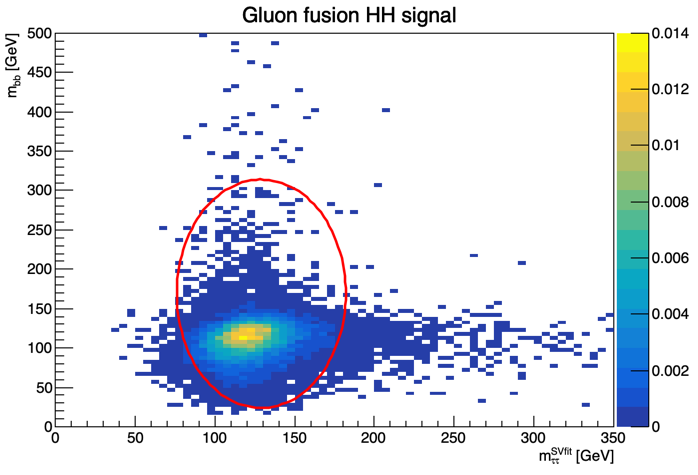
\includegraphics[width=0.45\textwidth]{Images/inclusive_2018_2b_Sig}}
	\subfloat{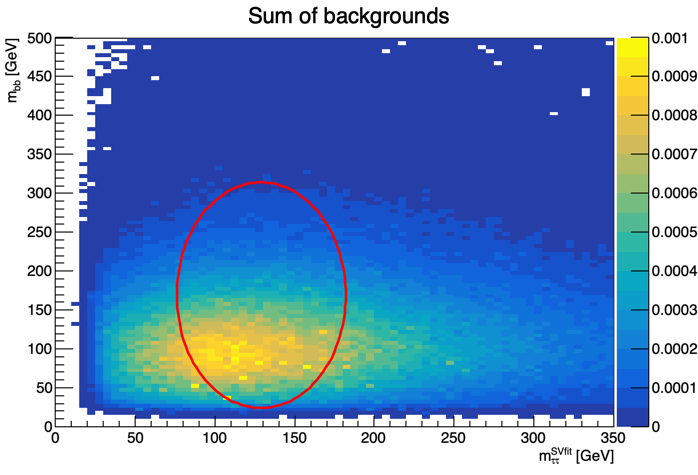
\includegraphics[width=0.45\textwidth]{Images/inclusive_2018_2b_Bkg}}
\end{center}
\caption{2D distributions of ($m_\text{bb}$, $m_{\tau\tau}$) for the HH SM ggHH signal (left) and the sum of backgrounds (right) for events belonging to the Resolved, 2 b-tag category and the three $\tau\tau$ channels considered for 2018. The red line shows the region selected by the resolved elliptical cut.}
\label{hh:fig:mass_cut}
\end{figure}


\subsection{Signal extraction}
\label{hh:subs:signal_extraction}

The eight orthogonal categories described in Section~\ref{hh:sec:event_categorization} are used for the signal extraction via a DNN developed to identify HH~$\to$~bb$\tau\tau$ events. The approach used to train the DNN \cite{hh:analysis:gilesdnn} follows the one used in the CMS di-Higgs HL-LHC projection analysis for the bb$\tau\tau$ channel \cite{hh:analysis:hh_hllhc}. The goal of the DNN is to classify events as originating either from signal (SM HH~$\to$bb$\tau\tau$ produced via ggHH) or background processes by assigning them a single prediction. Values closer to one indicates ``signal-like'' events, while  closer to zero, ``background-like'' events. The final DNN distributions obtained by inferring this network prediction in each category, $\tau\tau$ channel and year are the ones used in the signal extraction fit.

Training is performed with the \textsc{PyTorch} \cite{hh:analysis:pytorch} algorithm interfaced with \textsc{LUMIN} \cite{hh:analysis:lumin}. Events used for training are splitted in two halves. A pair of discriminators are then trained with each half of the data. At inference time, the discriminators are used to predict the classes of events in the halves of the data that were not used for the training. This way, all MC data can be used for the training without adding a bias on the predictions that would arise if only one network was used and the same data used for training was also used for inference. To further increase the statistical robustness, each discriminator consists of 10 neural networks, each trained with a different starting random seed.

For the training, a total of 26 features (selected among over a 100) are used as input to the neural network. Both categorical (year of data taking, the $\tau\tau$ decay mode or the number of VBF jet candidates) and object features are used. From the latter, the most important features (ranked by permutation importance) are the DeepJet scores of the b jets, the invariant masses of the bb, $\tau\tau$ and HH systems and kinematic variables of the reconstructed particles.



%%%%%%%%%%%%%%%%%%%%%%%%%%% MULTI-CLASS %%%%%%%%%%%%%%%%%%%%%%%%%%%%%%%%%

\subfile{multiclass}

%%%%%%%%%%%%%%%%%%%%%%%%%%%%%%%%%%%%%%%%%%%%%%%%%%%%%%%%%%%%%%%%%%%%%%%%%

\section{Background estimation}

%%%%%%%%%%%%%%%%%%%%%%%%%%%%%% QCD %%%%%%%%%%%%%%%%%%%%%%%%%%%%%%%%%%%%%%

\subfile{qcd}

%%%%%%%%%%%%%%%%%%%%%%%%%%%%%%%%%%%%%%%%%%%%%%%%%%%%%%%%%%%%%%%%%%%%%%%%%

\subsection{Z/$\gamma^*$~+~jets}
\label{hh:subs:dy}

The contribution of Z/$\gamma^*\to ll$ associated with jets is estimated from Monte-Carlo simulations. Samples can be produced with \textsc{MadGraph5\_aMC@NLO} at LO or NLO precisions. Sample generation with LO precision can be done in an inclusive way, with up to four jets produced at matrix element, or in different samples with different number of jets at matrix element (from one to four) or requiring two b jets. The combination of both inclusive and exclusive samples lead to large statistics for this process. However, LO modelling of the jets is not really good. NLO modelling leads to better results, although samples are only generated with up to two jets and no samples with two b jets are generated. Therefore, the lack of statistics makes NLO samples not useful. The final solution is use the samples with LO precision but improving the modelling by correcting the simulation with a data-driven method. The correction factors or \textit{scale factors} used in the MC samples are derived from several $Z\to\mu\mu$ sideband regions.

For the scale factor computation, events are required to pass a selection similar to the one applied in the analysis. At trigger level, events are selected by the single-muon trigger, with $p_T$ thresholds of 22~GeV in 2016 and 24~GeV in 2017 and 2018. At offline level, events should have two muons with $p_T > 20~$GeV and $|\eta|<2.4$ and one muon should match the muon used for triggering. A vertex constraint of $d_{xy} < 0.045~$mm and $d_z < 0.2~$mm is applied to both muons, and they should pass the tight muon identification and tight isolation working points. The selected muon pair should be separated by $\Delta R>0.1$, have opposite charge and an invariant mass of $m_{\mu\mu}>50~$GeV. The third lepton veto and the jet section are the same as for the analysis final states.

To reduce the QCD and t$\bar{\text{t}}$ contributions in the sideband region, a cut on the missing transverse energy is applied by requiring $E_T^{\text{miss}} < 45~$GeV.

Scale factors are estimated using 18 control regions. First, events are split in 3 regions based on the number of jets that pass the medium DeepJet b-tag working point: 0, 1 or 2. The latter is the one with the highest contribution, since it has exactly the same final state as the signal. Then, each control region is divided in six control regions based on the $p_T$ of the reconstructed Z candidate. The six control regions are named as \textit{Very Low $p_T$}, \textit{Low $p_T$}, \textit{Medium 1 $p_T$}, \textit{Medium 2 $p_T$}, \textit{High $p_T$} and \textit{Very High $p_T$}. The $p_T$ range of each control region varies with the year, as shown in Table~\ref{hh:tab:dy_sf}.

\begin{table}[h!]
\begin{center}
\begin{tabular}{c | c | c | c}
$p_T$ region & $p_T$ range - 2016 & $p_T$ range - 2017 & $p_T$
range - 2018 \\\hline
Very Low $p_T$  & $0<p_T\leq 10$    & $0<p_T\leq 10$    & $0<p_T\leq 10$     \\
Low $p_T$       & $10<p_T\leq 50$   & $10<p_T\leq 30$   & $10<p_T\leq 30$    \\
Medium 1 $p_T$  & $50<p_T\leq 80$   & $30<p_T\leq 50$   & $30<p_T\leq 50$    \\
Medium 2 $p_T$  & $80<p_T\leq 110$  & $50<p_T\leq 100$  & $50<p_T\leq 100$    \\
High $p_T$      & $110<p_T\leq 190$ & $100<p_T\leq 200$ & $100<p_T\leq 200$  \\
Very High $p_T$ & $p_T> 190$        & $p_T> 200$        & $p_T> 200$       
\end{tabular}
\caption{Definition of the Z $p_T$ regions for the Z/$\gamma^*\to ll$~+~jets scale factor computation.}
\label{hh:tab:dy_sf}
\end{center}
\end{table}

In each of the 18 regions, LO Z/$\gamma^*\to ll$ MC samples are subdivided in another 18 contributions, based on the number of b-partons at Matrix Element level (0, 1, 2) and the $p_T$ of the Z boson at generator level (same $p_T$ ranges as for the sideband regions). The data distribution of the invariant mass of the muon pair is fitted simultaneously in all categories, leaving the normalization of the DY contributions floating. The scale factors obtained are shown in Fig.~\ref{hh:fig:dy_sf}. Fig.~\ref{hh:fig:dy_sf_datamc} shows, as an example, how the distribution of $m_{\tau\tau}$ improves after applying the computed scale factors.


\begin{figure}[h!]
\begin{center}
\subfloat[2016]{\includegraphics[width=0.45\textwidth]{Images/SFs_2016}}
\subfloat[2017]{\includegraphics[width=0.45\textwidth]{Images/SFs_2017}}\\
\subfloat[2018]{\includegraphics[width=0.45\textwidth]{Images/SFs_2018}}
\end{center}
\caption{Scale factors, obtained from the simultaneous fit on $m_{\mu\mu}$ in 18 control regions for the 2016, 2017, and 2018 analyses.}
\label{hh:fig:dy_sf}
\end{figure}

\begin{figure}[h!]
\begin{center}
\subfloat{\includegraphics[width=0.45\textwidth]{Images/m_tt_vis_2btag_2018_noSF}}
\subfloat{\includegraphics[width=0.45\textwidth]{Images/m_tt_vis_2btag_2018}}
\end{center}
\caption{Distribution of $m_{\mu\mu}$ in the sideband region defined to compute the DY scale factors where the two jets pass the medium DeepJet working point. Left plot shows the distribution without applying the obtained scale factors; right plot after applying them.}
\label{hh:fig:dy_sf_datamc}
\end{figure}


\subsection{Top-antitop background}
\label{hh:subs:tt}

The contribution of the t$\bar{\text{t}}$ background is modelled relying on the MC simulation. However, while the shape of the process if well modelled by the simulation, the normalization of the background shows a disagreement with respect to the data, as can be seen in Fig.~\ref{hh:fig:ttbar_disc}.

\begin{figure}[h]
\begin{center}
\subfloat[]{\includegraphics[width=0.33\textwidth]{Images/dau1_eta_baseline_SR_MuTau}}
\subfloat[]{\includegraphics[width=0.33\textwidth]{Images/dau1_eta_baseline_SR_ETau}}
\subfloat[]{\includegraphics[width=0.33\textwidth]{Images/dau1_eta_baseline_SR_TauTau}}
\end{center}
\caption{Distributions of the $\eta$ of the first lepton in 2016 for the (a) \taumu\tauh{} channel, (b) \taue\tauh{} channel, and (c) \tauh\tauh{} channel. The two channels with the biggest t$\bar{\text{t}}$ contribution (\taumu\tauh{} and \taue\tauh{}) show a data/background agreement in the $\eta$ region where more t$\bar{\text{t}}$ is expected, while good agreement can be seen where poor contamination of t$\bar{\text{t}}$ is present, which points to an issue in the t$\bar{\text{t}}$ normalization.}
\label{hh:fig:ttbar_disc}
\end{figure}

In order to solve this normalization problem, a specific t$\bar{\text{t}}$ control region has been defined and fitted to extract an scale factor to be applied to the t$\bar{\text{t}}$ background yield. This control region had to be as close as possible to the signal region but orthogonal to it, group as many t$\bar{\text{t}}$ events as possible and the minimal from other backgrounds and cannot depend on the $\tau$ pair decay mode. The control region was finally defined by applying the same selections shown in Section~\ref{hh:sec:event_categorization} for the Resolved, 2 b-tag category except for the mass cut, which will be the inverse of the mass cut used in that category:
\begin{equation}
\frac{(m_{\tau\tau} - 129~\text{GeV})^2}{(53~\text{GeV})^2} + \frac{(m_\text{bb} - 169~\text{GeV})^2}{(145~\text{GeV})^2} > 1.
\end{equation}

A fit is performed in this region by including only as nuisance parameters (\textcolor{red}{these should be explained somewhere before}) this t$\bar{\text{t}}$ scale factor (that applies only to t$\bar{\text{t}}$ background) and the statistical uncertainties in each of the three years. The results are found in Table~\ref{hh:tab:ttsf}.

\begin{table}[h!]
\begin{center}
\begin{tabular}{c | c | c}
2016 & 2017 & 2018 \\
\hline
$0.908 \pm 0.006$ &  $0.988 \pm 0.006$ & $0.966 \pm 0.009$
\end{tabular}
\end{center}
\caption{Results of the t$\bar{\text{t}}$ control region fits for the three years. The values of the t$\bar{\text{t}}$ scale factors and their uncertainties are reported.}
\label{hh:tab:ttsf}
\end{table}


\subfile{corrections}

%\bibliographystyle{plain}
%\bibliography{../biblio.bib}


\end{document}

